\chapter{Solution to One-Variable Equation}

There are variety of ways to solve the scalar function $f(x)=0$ for independent variable $x$, the most intuitive of which being deriving its analytical solution in the explicit form. However, in many cases the explicit analytical solution of $x$ may not be achievable due to the complexity of $f(x)$. To address this problem, many numerical analysis based methods have been developed to obtain (an approximation of) the solution effectively and efficiently.

This chapter discusses these numerical methods as well as their convergence and computational burden. 

\section{Problem Formulation}

Let $f(x)=0$ be a scalar function, where $f(x)$ is continuous. There is at least one solution to $f(x)=0$, namely $p$, and $p\in \left[a, b\right]$. The target is to find $p$. A demonstrative plot is given in Fig. \ref{fig:part-5:onevarproblemformulation}. In the example, function $f(x)=0$ has two solutions within $\left[0, 10\right]$. The target is to find any one of them.

\begin{figure}[htbp]
\centering
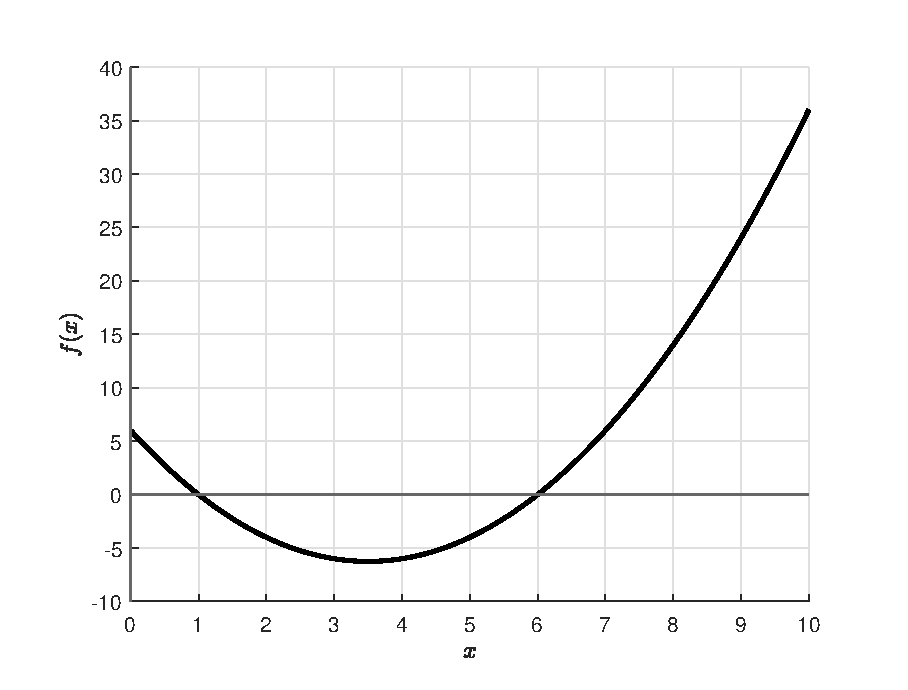
\includegraphics[width=250pt]{chapters/part-5/figures/demo_problem_formulation.eps}
\caption{A demonstrative example of solving $f(x)=0$ using numerical methods.} \label{fig:part-5:onevarproblemformulation}
\end{figure} 

Notice that there might be other solutions to $f(x)=0$ within $\left[a, b\right]$ than $p$. Useful it may be to find all solutions, however, in the scope of our discussion we look for only one solution. 

\subsection{Bisection Method}

Inspired by the \textit{intermediate value theorem}, so long as we can find an interval $\left[a, b\right]$ so that $f(a)f(b)<0$, we know that there must be a solution $p\in\left[a, b\right]$ such that $f(p)=0$. As long as we can narrow down the interval, we can approach the solution.

\begin{shortbox}
\Boxhead{Intermediate Value Theorem}

Let $f(x)$ be a continuous function whose domain contains the interval $\left[a, b\right]$. Without loosing generality, let us assume that $f(a)<f(b)$. Then $\forall c \in \left[f(a), f(b)\right]$, $\exists x_0 \in \left[a, b\right]$, so that $f(x_0)=c$.

\end{shortbox}

The algorithm is summarized as follows. Let $f(x)$ be a continuous function on $\left[a, b\right]$, and $f(a)f(b)<0$. Do the following to find a solution $f(p)=0$ within $\left[a, b\right]$.

\begin{enumerate}
\item Let $a_1 = a$, $b_1=b$.
\item Let $p_i = \frac{a_i+b_i}{2}$.
\item Calculate $f(p_i)$. If $f(p_i)=0$, then $p_i$ is a solution. Otherwise:
\begin{itemize}
  \item If $f(p_i)f(a_i) < 0$, let $a_{i+1}=a_i, b_{i+1}=p_i$.
  \item If $f(p_i)f(b_i) < 0$, let $a_{i+1}=p_i, b_{i+1}=b_i$.
\end{itemize}
\item Iterate from Step 2.
\end{enumerate}